{
For at beskrive integrationen og samspillet mellem en kørsel og
databasen vil der følge en beskrivelse af de vigtige kald mellem 
start.py og databasen. 
%intro til start.py
\subsection{Workflow}
%find på en bedre titel!
Start.py er distributør af arbejde til de andre dele af programkoden.
Diagram \ref{start_workflow} og pseudokode \ref{pseudo_workflow} giver et overblik over hvad der bliver
forklaret i resten af dette kapitel. 
\begin{figure}[h!]
	\begin{center}
		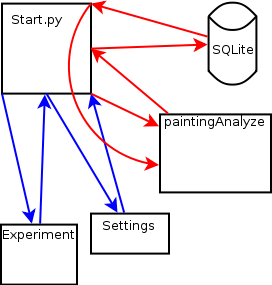
\includegraphics[scale=0.5]{afsnit/implementation/billeder/workflow_start_py.png}
	\end{center}
	\caption{De blå pile er ting, som sker en enkelt gang, mens de blå
	\label{start_workflow}
	bliver gentaget indtil der ikke er flere billeder at arbejde på}
\end{figure}
\begin{lstlisting}[caption={Pseudokode for
start},frame=tb,label={pseudo_workflow}]
cuts = experiment.generateCuts()
experiment.setSettings(settings)
experiment.setGlobalSettings(globalSettings)
db = Database(globalSettings)
run = m.createNewRun(settings)
paintings = m.Painting.select(m.Painting.q.form=="painting")
for painting in paintings:
	paintingContainer = Painting(painting)
	paintingContainer.setResults(paintingAnalyzer.analyze(paintingContainer,settings))
	m.saveResults(run.id,paintingContainer)
\end{lstlisting}
\subsubsection{Eksperimenter}
Eksperimenterne er til for at samle konfigurationen af en kørsel.
Kravene til et eksperiment er at den skal have mindst tre metoder:
generation af snit, sætte globale indstillinger samt sætte
kørselsspecifikke indstillinger. \ref{pseudo_experiment} er et eksempel
på hvordan et eksperiment evt. kunne se ud.
\begin{lstlisting}[caption={Pseudokode for et
experiment, som checker på $\varPhi$},frame=tb,label={pseudo_experiment}]
def generateCuts():
	cuts = [goldenLibrary.PHI,2/3]
	return cuts
def setSettings(settings):
	settings.setMarginPercentage(0.024)
	return 0
def setGlobalSettings(globalSettings):
	return 0
\end{lstlisting}
%Settings 
\subsubsection{Globale indstillinger}
Globale indstillinger er informationer, som har brug for at blive gemt
mellem kørsler. I det nuværende tilfælde er det placeringen på databasen og
csvfilen fra wga.hu, det kunne udvides til også at inkludere placeringen
af billederne istedet for at være fastdefineret.
\subsubsection{Initiallisering af databasen}
%konstruktion af databasen inklusiv downloading og crawling

\subsubsection{Kørselsindstillinger}
Disse indstilinger kan afvige i forskellige kørsler, det er variable
hvis indstillinger betyder meget for resultaterne og derfor er vigtige
at kunne ændre. De består af tærskelværdier for floodfill og
kantdetektion samt størrelsen på margin\ref{tærskelværdi}, de snit, som
skal undersøges og hvilken metode, der skal benyttes.
%Loop
}
% vim: set tw=72 spell spelllang=da:
